\documentclass[11pt,]{article}
\usepackage[left=1in,top=1in,right=1in,bottom=1in]{geometry}
\newcommand*{\authorfont}{\fontfamily{phv}\selectfont}
\usepackage[]{mathpazo}


  \usepackage[T1]{fontenc}
  \usepackage[utf8]{inputenc}



\usepackage{abstract}
\renewcommand{\abstractname}{}    % clear the title
\renewcommand{\absnamepos}{empty} % originally center

\renewenvironment{abstract}
 {{%
    \setlength{\leftmargin}{0mm}
    \setlength{\rightmargin}{\leftmargin}%
  }%
  \relax}
 {\endlist}

\makeatletter
\def\@maketitle{%
  \newpage
%  \null
%  \vskip 2em%
%  \begin{center}%
  \let \footnote \thanks
    {\fontsize{18}{20}\selectfont\raggedright  \setlength{\parindent}{0pt} \@title \par}%
}
%\fi
\makeatother




\setcounter{secnumdepth}{0}

\usepackage{color}
\usepackage{fancyvrb}
\newcommand{\VerbBar}{|}
\newcommand{\VERB}{\Verb[commandchars=\\\{\}]}
\DefineVerbatimEnvironment{Highlighting}{Verbatim}{commandchars=\\\{\}}
% Add ',fontsize=\small' for more characters per line
\usepackage{framed}
\definecolor{shadecolor}{RGB}{248,248,248}
\newenvironment{Shaded}{\begin{snugshade}}{\end{snugshade}}
\newcommand{\KeywordTok}[1]{\textcolor[rgb]{0.13,0.29,0.53}{\textbf{#1}}}
\newcommand{\DataTypeTok}[1]{\textcolor[rgb]{0.13,0.29,0.53}{#1}}
\newcommand{\DecValTok}[1]{\textcolor[rgb]{0.00,0.00,0.81}{#1}}
\newcommand{\BaseNTok}[1]{\textcolor[rgb]{0.00,0.00,0.81}{#1}}
\newcommand{\FloatTok}[1]{\textcolor[rgb]{0.00,0.00,0.81}{#1}}
\newcommand{\ConstantTok}[1]{\textcolor[rgb]{0.00,0.00,0.00}{#1}}
\newcommand{\CharTok}[1]{\textcolor[rgb]{0.31,0.60,0.02}{#1}}
\newcommand{\SpecialCharTok}[1]{\textcolor[rgb]{0.00,0.00,0.00}{#1}}
\newcommand{\StringTok}[1]{\textcolor[rgb]{0.31,0.60,0.02}{#1}}
\newcommand{\VerbatimStringTok}[1]{\textcolor[rgb]{0.31,0.60,0.02}{#1}}
\newcommand{\SpecialStringTok}[1]{\textcolor[rgb]{0.31,0.60,0.02}{#1}}
\newcommand{\ImportTok}[1]{#1}
\newcommand{\CommentTok}[1]{\textcolor[rgb]{0.56,0.35,0.01}{\textit{#1}}}
\newcommand{\DocumentationTok}[1]{\textcolor[rgb]{0.56,0.35,0.01}{\textbf{\textit{#1}}}}
\newcommand{\AnnotationTok}[1]{\textcolor[rgb]{0.56,0.35,0.01}{\textbf{\textit{#1}}}}
\newcommand{\CommentVarTok}[1]{\textcolor[rgb]{0.56,0.35,0.01}{\textbf{\textit{#1}}}}
\newcommand{\OtherTok}[1]{\textcolor[rgb]{0.56,0.35,0.01}{#1}}
\newcommand{\FunctionTok}[1]{\textcolor[rgb]{0.00,0.00,0.00}{#1}}
\newcommand{\VariableTok}[1]{\textcolor[rgb]{0.00,0.00,0.00}{#1}}
\newcommand{\ControlFlowTok}[1]{\textcolor[rgb]{0.13,0.29,0.53}{\textbf{#1}}}
\newcommand{\OperatorTok}[1]{\textcolor[rgb]{0.81,0.36,0.00}{\textbf{#1}}}
\newcommand{\BuiltInTok}[1]{#1}
\newcommand{\ExtensionTok}[1]{#1}
\newcommand{\PreprocessorTok}[1]{\textcolor[rgb]{0.56,0.35,0.01}{\textit{#1}}}
\newcommand{\AttributeTok}[1]{\textcolor[rgb]{0.77,0.63,0.00}{#1}}
\newcommand{\RegionMarkerTok}[1]{#1}
\newcommand{\InformationTok}[1]{\textcolor[rgb]{0.56,0.35,0.01}{\textbf{\textit{#1}}}}
\newcommand{\WarningTok}[1]{\textcolor[rgb]{0.56,0.35,0.01}{\textbf{\textit{#1}}}}
\newcommand{\AlertTok}[1]{\textcolor[rgb]{0.94,0.16,0.16}{#1}}
\newcommand{\ErrorTok}[1]{\textcolor[rgb]{0.64,0.00,0.00}{\textbf{#1}}}
\newcommand{\NormalTok}[1]{#1}

\usepackage{graphicx}
% We will generate all images so they have a width \maxwidth. This means
% that they will get their normal width if they fit onto the page, but
% are scaled down if they would overflow the margins.
\makeatletter
\def\maxwidth{\ifdim\Gin@nat@width>\linewidth\linewidth
\else\Gin@nat@width\fi}
\makeatother
\let\Oldincludegraphics\includegraphics
\renewcommand{\includegraphics}[1]{\Oldincludegraphics[width=\maxwidth]{#1}}

\title{Implementing Option Pricing Model  }



\author{\Large Zhao Ming\vspace{0.05in} \newline\normalsize\emph{Utah State University}  }


\date{}

\usepackage{titlesec}

\titleformat*{\section}{\normalsize\bfseries}
\titleformat*{\subsection}{\normalsize\itshape}
\titleformat*{\subsubsection}{\normalsize\itshape}
\titleformat*{\paragraph}{\normalsize\itshape}
\titleformat*{\subparagraph}{\normalsize\itshape}


\usepackage{natbib}
\bibliographystyle{apsr}



\newtheorem{hypothesis}{Hypothesis}
\usepackage{setspace}

\makeatletter
\@ifpackageloaded{hyperref}{}{%
\ifxetex
  \usepackage[setpagesize=false, % page size defined by xetex
              unicode=false, % unicode breaks when used with xetex
              xetex]{hyperref}
\else
  \usepackage[unicode=true]{hyperref}
\fi
}
\@ifpackageloaded{color}{
    \PassOptionsToPackage{usenames,dvipsnames}{color}
}{%
    \usepackage[usenames,dvipsnames]{color}
}
\makeatother
\hypersetup{breaklinks=true,
            bookmarks=true,
            pdfauthor={Zhao Ming (Utah State University)},
             pdfkeywords = {Monte Carlo, control variates, option pricing},  
            pdftitle={Implementing Option Pricing Model},
            colorlinks=true,
            citecolor=blue,
            urlcolor=blue,
            linkcolor=magenta,
            pdfborder={0 0 0}}
\urlstyle{same}  % don't use monospace font for urls



\begin{document}
	
% \pagenumbering{arabic}% resets `page` counter to 1 
%
% \maketitle

{% \usefont{T1}{pnc}{m}{n}
\setlength{\parindent}{0pt}
\thispagestyle{plain}
{\fontsize{18}{20}\selectfont\raggedright 
\maketitle  % title \par  

}

{
   \vskip 13.5pt\relax \normalsize\fontsize{11}{12} 
\textbf{\authorfont Zhao Ming} \hskip 15pt \emph{\small Utah State University}   

}

}







\begin{abstract}

    \hbox{\vrule height .2pt width 39.14pc}

    \vskip 8.5pt % \small 

\noindent In this paper I replicate Clewlow and Strickland's control variates
methods based on Greek letters method to test if it can improve the
simulation efficiency. First, I use Black Scholes Merton formula for
option pricing as a benchmark, to compare with the Euorpean call option
price from Monte Carlo methods. Then I use Greek letters as control
variates to reduce sample standard deviation and improve the efficiency
of the Monte Carlo simulation. The whole process is programming in C++.
C++ is a compiled language which can generate machine code from source
code and provide a shorter running time. This paper is based on ideas
from \emph{Implementing Derivatives Models} by Clewlow and Strickland,
\emph{On The Simulation of Contingent Claims} by Clewlow and Carverhill,
Chapter 4, and \emph{Derivatives Markets} by McDonald, Chapter 12, 13,
19.


\vskip 8.5pt \noindent \emph{Keywords}: Monte Carlo, control variates, option pricing \par

    \hbox{\vrule height .2pt width 39.14pc}



\end{abstract}


\vskip 6.5pt

\noindent \doublespacing \section{Introduction}\label{introduction}

Black-Scholes Merton formula is used to compute the theoretical price of
the European call option for a stock under certain assumptions. Monte
Carlo method is based on random sampling to generate the numerical
results. We chose to use Black-Scholes Merton formula as a benchmark to
find the option price, then simulate the option price using Monte Carlo
method, comparing with the two results to evaluate if Monte Carlo method
could provide a correct option price. Next, we combine Greek letters
with Monte Carlo method, calculate the standard errors from both
Delta-hedging Monte Carlo, Delta-Gamma hedging Monte Carlo and naive
Monte Carlo to test how control variates reduce the standard deviation
and improve the efficiency of Monte Carlo simulation. At the end, we
switch from Black-Scholes Merton's world to Jump world which imitates
the real world and test control variates method.

\section{Section 1 Control Variates}\label{section-1-control-variates}

The control variates method is a variance reduction technique that is
used in the Monte Carlo simulation algorithms. It can help to reduce the
standard error of an estimate of an unknown quantity, and improve the
efficiency of the simulation.

\citet{ClewlowandCarverhill} mention in their paper, ``the control
variate is a known value that is closely related to the unknown quantity
to be simulated. A good control variate for an option problem might be
the price of a similar type of option for which an analytic valuation
equation exists. The simulation will estimate the difference between the
unknown value and the control variate, and this gives a greater accuracy
than the unknown value itself. The control variates are intimately
related to the hedging of the option. The control Variates are not only
improving efficiency but can also providing insights into the hedging of
the option'' (ClewlowStrickland).

\citet{McDonald} presents an example of pricing an arithmetic Asian call
option. He suggests using a geometric Asian option as the control
variate. There is a convenient closed-form solution that is a special
case of the Black-Scholes Merton formula for options with a geometric
mean payoff function. He combines this with a Monte Carlo estimate of
the known geometric Asian option, and thereby can compute an estimated
sampling error along each path. McDonald reports significant variance
reduction in the Monte Carlo sampling routine for the arithmetic Asian
option.

The underlying method is to estimate the error of each trial by using
the price of a related option that does have a pricing formula. The
error estimate obtain from this control price can be used to improve the
accuracy of the Monte Carlo price on each trial.

Because we are using the same random numbers to estimate the option, the
errors in the estimated arithmetic and geometric prices are correlated.
When the estimated price for the geometric option is high, it should
have a high arithmetic price as well. We can use information on the
error in the geometric price to adjust our estimate of the arithmetic
price.

\[
A^* = \bar A + \beta(G-\bar G)
\]

In formula above, we estimate both arithmetic price, \(\bar A\) and
geometric price, \(\bar G\). And ``A'' and ``G'' represent the true
arithmetic and geometric prices. The error term from the Monte Carlo
estimates the geometric price is \((G - \bar G)\). We want to use this
error to improve our estimate of the arithmetic price.

We could find an optimized \(\beta\) to help better estimate \(A^*\)

As \citet{ClewlowStrickland} point out, looking to hedging instruments
that reduce the variance of overall portfolio cash-flow variance turns
out to be an excellent strategy for identifying valid control variates.
As such, they employ the Delta and Gamma from the well-known
Black-Scholes Merton model. Considering when they sold a call option,
when the stock price increases, they would lose lots of money, because
the customer would execute the call option. The Market-maker will have a
large standard deviation in their whole portfolio. Instead,
Market-makers could buy Delta shares when they sold a call option, if
the stock price went up, they could sell those shares to customers when
they bought at a lower price. If the stock price decreases, the
customers would not execute the option, so Market-makers could keep the
premium. When the Market-makers applied Delta and Gamma for control
variates, they will reduce their portfolio's sample variance.

\begin{figure}
\centering
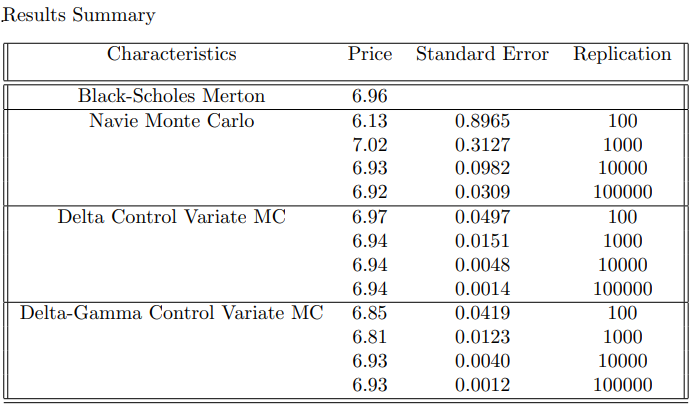
\includegraphics{images/Result.PNG}
\caption{This is the result by comparing Blach-Schoels Merton option
price with Monte Carlo methods.}
\end{figure}

\section{Section 2 Black-Scholes Merton
model}\label{section-2-black-scholes-merton-model}

This is Black-Scholes Merton formula for a European call option.

\[
C(S, K, \sigma,r, T, \delta) = S e^{-\delta T} N(d_{1}) - K e^{-r T} N(d_{2})
\] \[
d_{1} = \frac{\ln{(S/K)} + (r - \delta + \frac{1}{2} \sigma^{2}) T}{\sigma \sqrt{T}} 
\] \[
d_{2} = d_{1} - \sigma \sqrt{T}
\] In Black-Scholes Merton formula, we can interpret Delta as a
share-equivalent. Black-Scholes Merton formula tells us both option
price and what position in the stock is equivalent to the option.

\citet{McDonald} points out ``Black-Scholes Merton formula is
constrained by certain economic environment, the risk-free rate is known
and constant, there are no transaction costs, and it is possible to
short-sell costlessly and to borrow at the risk-free rate'' (McDonald).

Monte Carlo simulation is to obtain the option price for models that do
not have analytical formulas; it can also simulate asset path with
stochastic volatility.

\begin{Shaded}
\begin{Highlighting}[]
\DataTypeTok{double}\NormalTok{ blackScholesCall(}\AttributeTok{const} \DataTypeTok{double}\NormalTok{& spot, }\AttributeTok{const} \DataTypeTok{double}\NormalTok{& strike, }\AttributeTok{const} \DataTypeTok{double}\NormalTok{& vol}
\NormalTok{                        , }\AttributeTok{const} \DataTypeTok{double}\NormalTok{& rate,}\AttributeTok{const} \DataTypeTok{double}\NormalTok{& expiry, }\AttributeTok{const} \DataTypeTok{double}\NormalTok{& div)}
\NormalTok{\{}
    \KeywordTok{auto}\NormalTok{ d1 = (}\BuiltInTok{std::}\NormalTok{log(spot / strike) + (rate - div + }\FloatTok{0.5}\NormalTok{ * vol * vol) * expiry) }
\NormalTok{            / (vol * }\BuiltInTok{std::}\NormalTok{sqrt(expiry));}
    \KeywordTok{auto}\NormalTok{ d2 = d1 - (vol * }\BuiltInTok{std::}\NormalTok{sqrt(expiry));}
    \KeywordTok{auto}\NormalTok{ callPrc = (spot * }\BuiltInTok{std::}\NormalTok{exp(-div * expiry) * normalCDF(d1)) }
\NormalTok{                  - (strike * }\BuiltInTok{std::}\NormalTok{exp(-rate * expiry) * normalCDF(d2));}

    \ControlFlowTok{return}\NormalTok{ callPrc;}
\NormalTok{\}}
\end{Highlighting}
\end{Shaded}

In the code above, we define a function named ``blackScholesCall'', and
we pass information as parameters. Parameters are specified inside the
parentheses, and you can add as many as you want, like here, we include
all the variables from the Black-Scholes Merton formula, and specify
variables' types before using them.

\(N(d_1)\) and \(N(d_2)\) are matching with normalCDF(d1) and
normalCDF(d2), which stands the cumulative normal distribution function,
showing the probability that a number randomly drawn from a standard
normal distribution will be less than \(d_1\) and \(d_2\).

From the ``blackScholesCall'' function, we could change the values of
parameters that are passing to the function and generate different
prices of call option.

\section{Section 3 Greeks with purposes of heding Versus Greeks for
control
variates}\label{section-3-greeks-with-purposes-of-heding-versus-greeks-for-control-variates}

Before talking about the Greeks, we want to mention what are
market-makers. Market-makers are the people or agents that are trading
with the customers. Market-makers maintain inventories to satisfy the
customers immediately. Market-makers make profits from bid-ask spread.
Also, market-makers could short-sell by borrowing other people's shares
and then selling those shares to generate inventory as needed.

Under unhedged situation, Market-makers will face the risk from the
adverse price movement. At the worst situation, unhedged position will
lead to bankruptcy.

Market-makers could use Delta-hedging to control risk. Market-makers
could compute the Delta value and buy Delta number of shares to offset
risk, market-makers need to invest capital to maintain a Delta-hedging
position because the cost of option is different from the cost of stock.

Delta measures the option price changes when stock price changes, also
Delta represents number of shares in the portfolio that replicates the
option.

\[
Call Delta= \frac{\partial C(S, K, \sigma, r, T - t, \delta)}{\partial S} = e^{-\delta (T - t)} N(d_{1}) 
\]

\begin{Shaded}
\begin{Highlighting}[]
\DataTypeTok{double}\NormalTok{ BlackScholesDelta(}\AttributeTok{const} \DataTypeTok{double}\NormalTok{& spot, }\AttributeTok{const} \DataTypeTok{double}\NormalTok{& t, }\AttributeTok{const} \DataTypeTok{double}\NormalTok{& strike,}
    \AttributeTok{const} \DataTypeTok{double}\NormalTok{& expiry, }\AttributeTok{const} \DataTypeTok{double}\NormalTok{& vol, }\AttributeTok{const} \DataTypeTok{double}\NormalTok{& rate, }\AttributeTok{const} \DataTypeTok{double}\NormalTok{& div)}
\NormalTok{\{}
    \KeywordTok{auto}\NormalTok{ tau = expiry - t;}
    \KeywordTok{auto}\NormalTok{ d1 = (}\BuiltInTok{std::}\NormalTok{log(spot / strike) + (rate - div + }\FloatTok{0.5}\NormalTok{ * vol * vol) * tau) }
\NormalTok{              / (vol * }\BuiltInTok{std::}\NormalTok{sqrt(tau));}
    \KeywordTok{auto}\NormalTok{ delta = }\BuiltInTok{std::}\NormalTok{exp(-div * tau) * normalCDF(d1);}

    \ControlFlowTok{return}\NormalTok{ delta;}
\NormalTok{\}}
\end{Highlighting}
\end{Shaded}

For a call option, Delta is positive. When the stock price increases,
the call option price will increase. The Delta will approach 1 when the
stock price is deep in the money. It shows the share-equivalent of the
option is 1.

Gamma shows the rate change of Delta when stock price changes by 1
dolloar.

\[
Call Gamma=  \frac{\partial^{2} C(S, K, \sigma, r, T - t, \delta)}{\partial S^{2}} = \frac{e^{-\delta (T - t)} N^{\prime}(d_{1})}{S \sigma \sqrt{T - t}} 
\]

\begin{Shaded}
\begin{Highlighting}[]
\DataTypeTok{double}\NormalTok{ BlackScholesGamma(}\AttributeTok{const} \DataTypeTok{double}\NormalTok{& spot, }\AttributeTok{const} \DataTypeTok{double}\NormalTok{& t, }\AttributeTok{const} \DataTypeTok{double}\NormalTok{& strike,}
    \AttributeTok{const} \DataTypeTok{double}\NormalTok{& expiry, }\AttributeTok{const} \DataTypeTok{double}\NormalTok{& vol, }\AttributeTok{const} \DataTypeTok{double}\NormalTok{& rate, }\AttributeTok{const} \DataTypeTok{double}\NormalTok{& div)}
\NormalTok{\{}
    \KeywordTok{auto}\NormalTok{ tau = expiry - t;}
    \KeywordTok{auto}\NormalTok{ d1 = (}\BuiltInTok{std::}\NormalTok{log(spot / strike) + (rate - div + }\FloatTok{0.5}\NormalTok{ * vol * vol) * tau) }
\NormalTok{              / (vol * }\BuiltInTok{std::}\NormalTok{sqrt(tau));}
    \KeywordTok{auto}\NormalTok{ gamma = (}\BuiltInTok{std::}\NormalTok{exp(-div * tau) * normpdf(d1) / (spot * vol * }\BuiltInTok{std::}\NormalTok{sqrt(tau)));}

    \ControlFlowTok{return}\NormalTok{ gamma;}
\NormalTok{\}}
\end{Highlighting}
\end{Shaded}

Delta alone is not predating the option price accurately because Delta
changes with the stock price. Delta will underestimate the actual change
when underlying asset price increases and overestimate the decline when
the stock price decreases. We add Gamma to improve it.

``The changes in the Delta and Gamma as the stock price evolves randomly
exactly offset the changes in the option value due to the random changes
in the stock price'' (ClewlowStrickland), delta and gamma provide good
results for hedging purposes, this is the reason why authors choose
Delta and Gamma for control variates in a numerical way.

\[
C(S_{t+h} )= C(S_t) + \epsilon \Delta(S_t) + \frac{1}{2}\epsilon^2\Gamma(S_t))
\]

The Delta approximation is a straight-line tangent to the option price
curve and is always below the option price curve. The Delta-Gamma
approximation uses the squared stock price change, which generates a
curve more closely approximating the option price curve. Using hedges as
control variates was first described by Clewlow and Carverhill. When
pricing a European call option, the distribution of the pay-off has a
large standard deviation. If we want to estimate the call value as the
mean of a number of Monte Carlo simulations then standard error of the
mean will be large. When using Delta control variate, the pay-off of the
hedged portfolio has a much smaller standard deviation.

\[
C_{t_0}e^{r(T-t_0)} = C_T - [\sum^{N-1}_{i=0}\frac{\partial C_{t_i}}{\partial S}(S_{t{_i+1}} - E[S_{t_i}])e^{r(T-t_{i+1})}] + \eta
\]

\section{Section 4 Variance
Reduction}\label{section-4-variance-reduction}

The main purpose for the Delta-hedging is to help market-makers to
maintain a Delta-neutral position, market-makers sell one call option
and hedges the position with shares.

And now from Clewlow and Carverhill, we are going to see how they using
Greeks as control variates to reduce the standard deviation and improve
the efficiency.

\begin{figure}
\centering
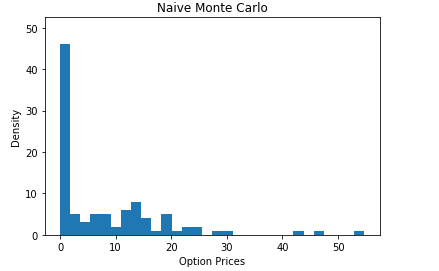
\includegraphics{images/Naive.PNG}
\caption{This is the call payoff from Monte Carlo simulation, used 252
time steps, and 100 simulations.}
\end{figure}

\begin{figure}
\centering
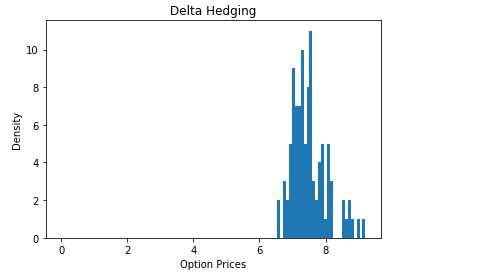
\includegraphics{images/DeltaHedging.PNG}
\caption{This is the call payoff from Delta-Hedged Monte Carlo
simulation, used 252 time steps, and 100 simulations.}
\end{figure}

\begin{figure}
\centering
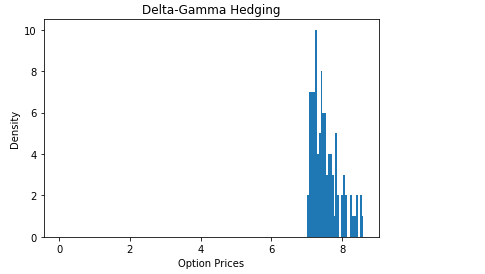
\includegraphics{images/DeltaGammaHedging.PNG}
\caption{This is the call payoff from Delta-Hedged Monte Carlo
simulation, used 252 time steps, and 100 simulations.}
\end{figure}

From the graph above, we could easily find after using Delta as control
variate, the result of call payoff has an obvious improvement. The
sample has a smaller standard deviation, and after using Delta-Gamma as
control variates, the standard deviation even gets smaller. If you only
using Monte Carlo simulation without control variates, you will need a
100 times larger sample size to get the standard deviation as same as
the Delta-hedging Monte Carlo.

We use the Monte Carlo method to simulate the discrete time asset paths
for the underlying asset.

\[
S_{t+h} = S_{t} e^{\{(r - \delta - \frac{1}{2} \sigma^{2}) h + \sigma \sqrt{h} z\}}
\]

\begin{Shaded}
\begin{Highlighting}[]
\BuiltInTok{std::}\NormalTok{vector<}\DataTypeTok{double}\NormalTok{> simulateNvPath(}\AttributeTok{const} \DataTypeTok{double}\NormalTok{& spot, }\AttributeTok{const} \DataTypeTok{double}\NormalTok{& rate, }\AttributeTok{const} \DataTypeTok{double}\NormalTok{& vol, }
                                   \AttributeTok{const} \DataTypeTok{double}\NormalTok{& div, }\AttributeTok{const} \DataTypeTok{double}\NormalTok{& expiry, }\AttributeTok{const} \DataTypeTok{size_t}\NormalTok{& numSteps)}
\NormalTok{\{}
    \KeywordTok{auto}\NormalTok{ dt = expiry / numSteps;}
    \KeywordTok{auto}\NormalTok{ nudt = (rate - div - }\FloatTok{0.5}\NormalTok{ * vol * vol) * dt;}
    \KeywordTok{auto}\NormalTok{ sigdt = vol * }\BuiltInTok{std::}\NormalTok{sqrt(dt);}
    \KeywordTok{auto}\NormalTok{ z = }\BuiltInTok{std::}\NormalTok{vector<}\DataTypeTok{double}\NormalTok{>(numSteps, }\FloatTok{0.0}\NormalTok{);}
    \KeywordTok{auto}\NormalTok{ path = }\BuiltInTok{std::}\NormalTok{vector<}\DataTypeTok{double}\NormalTok{>(numSteps, spot);}
\NormalTok{    RandomNormals(z);}

    \ControlFlowTok{for}\NormalTok{ (}\KeywordTok{auto}\NormalTok{ i = }\DecValTok{1}\NormalTok{; i < numSteps; ++i)}
\NormalTok{    \{}
\NormalTok{        path[i] = path[i - }\DecValTok{1}\NormalTok{] * }\BuiltInTok{std::}\NormalTok{exp(nudt + sigdt * z[i]);}
\NormalTok{    \}}

    \ControlFlowTok{return}\NormalTok{ path;}
\NormalTok{\}}
\end{Highlighting}
\end{Shaded}

In our code, we used ``dt'' to represent each time steps instead of
``h'' in the formula to represent the discrete intervals; ``z'' is
represented the generated random numbers which are normally distributed,
and help with simulating the random stock price for each time step. And
we used ``path'' to indicate the spot price. After that, we called the
call payoff function to get the payoff for each simulation.

\begin{Shaded}
\begin{Highlighting}[]
\KeywordTok{auto}\NormalTok{ callPayoff(}\AttributeTok{const} \DataTypeTok{double}\NormalTok{& spot, }\AttributeTok{const} \DataTypeTok{double}\NormalTok{& strike)}
\NormalTok{\{}
    \ControlFlowTok{return} \BuiltInTok{std::}\NormalTok{max(spot - strike, }\FloatTok{0.0}\NormalTok{);}
\NormalTok{\}}
\end{Highlighting}
\end{Shaded}

\[
\hat{C_0} = exp(-rT)\frac{1}{M}\sum^M_{j=1} max(0, S_{T,j} - K)
\]

We sum the pay-offs of each simulation, average them, then discounted
the average back to the present value. This is similar to the Law of
large numbers theory; the expected option price of some random payoff
can be approximated by taking the average of the random variables.

\subsection{Subsection A Delta control
variate}\label{subsection-a-delta-control-variate}

\[
cv_1 = \sum^{N-1}_{i=0} \frac{\partial C_{t_i}}{\partial S}(S_{t_{i+1}}-E[S_{t_i}])e^{r(T-t_{i+1})}
\]

\begin{Shaded}
\begin{Highlighting}[]
\ControlFlowTok{for}\NormalTok{ (}\KeywordTok{auto}\NormalTok{ i = }\DecValTok{1}\NormalTok{; i < numSteps; ++i)}
\NormalTok{    \{}
\NormalTok{        path[i] = path[i - }\DecValTok{1}\NormalTok{] * }\BuiltInTok{std::}\NormalTok{exp(nudt + sigdt * z[i]);}
        \KeywordTok{auto}\NormalTok{ t = i * dt;}
\NormalTok{        delta[i] = BlackScholesDelta(path[i - }\DecValTok{1}\NormalTok{], t, strike, expiry, vol, rate, div);}
\NormalTok{        cv1 += delta[i] * (path[i] - path[i - }\DecValTok{1}\NormalTok{] * erddt);}
\NormalTok{    \}}

\ControlFlowTok{for}\NormalTok{ (}\KeywordTok{auto}\NormalTok{ i = }\DecValTok{0}\NormalTok{; i < numReps; ++i)}
\NormalTok{    \{}
        \KeywordTok{auto}\NormalTok{ result = simulateDeltaHedgedPath(spot, rate, vol, div, expiry, numSteps, strike);}
        \KeywordTok{auto}\NormalTok{ spotT = }\BuiltInTok{std::}\NormalTok{get<}\DecValTok{0}\NormalTok{>(result);}
        \KeywordTok{auto}\NormalTok{ cv1 = }\BuiltInTok{std::}\NormalTok{get<}\DecValTok{1}\NormalTok{>(result);}
\NormalTok{        callPrice += callPayoff(spotT, strike) + beta1 * cv1;}
\NormalTok{    \}}
\end{Highlighting}
\end{Shaded}

From the first ``for loop'' in the code above, we calculate the Delta
for each time step from the Black-Scholes Delta formula. Delta will
rebalance discretely for each step for every simulation. We will get a
Delta for each time step. And then using the Delta to get the value of
control variates. The authors choose the beta1 = -1 which is the
appropriate value for this example where they have the exact Delta. The
variable ``erddt'' allow us to compute \(E[S_{t_{i+1}}]\) efficiently.

\subsection{Subsection B Delta-Gamma control
variates}\label{subsection-b-delta-gamma-control-variates}

\[
cv_2 = \sum^{N-1}_{i=0} \frac{\partial^2 C_{t_i}}{\partial S^2}((\Delta S_{t_i})^2 - E[(\Delta S_{t_i})^2])e^{r(T-t_{i+1})}
\]

\begin{Shaded}
\begin{Highlighting}[]
\ControlFlowTok{for}\NormalTok{ (}\KeywordTok{auto}\NormalTok{ i = }\DecValTok{1}\NormalTok{; i < numSteps; ++i)}
\NormalTok{    \{}
\NormalTok{        path[i] = path[i - }\DecValTok{1}\NormalTok{] * }\BuiltInTok{std::}\NormalTok{exp(nudt + sigdt * z[i]);}
        \KeywordTok{auto}\NormalTok{ t = i * dt;}
\NormalTok{        delta[i] = BlackScholesDelta(path[i - }\DecValTok{1}\NormalTok{], t, strike, expiry, vol, rate, div);}
\NormalTok{        gamma[i] = BlackScholesGamma(path[i - }\DecValTok{1}\NormalTok{], t, strike, expiry, vol, rate, div);}
\NormalTok{        cv1 += delta[i] * (path[i] - path[i - }\DecValTok{1}\NormalTok{] * errdt);}
\NormalTok{        cv2 += gamma[i] * ((path[i] - path[i - }\DecValTok{1}\NormalTok{]) * (path[i] - path[i - }\DecValTok{1}\NormalTok{]) }
\NormalTok{                       - path[i - }\DecValTok{1}\NormalTok{] * path[i - }\DecValTok{1}\NormalTok{] * egamma);}
\NormalTok{    \}}

\ControlFlowTok{for}\NormalTok{ (}\KeywordTok{auto}\NormalTok{ i = }\DecValTok{0}\NormalTok{; i < numReps; ++i)}
\NormalTok{    \{}
        \KeywordTok{auto}\NormalTok{ result = simulateDeltaGammaHedgedPath(spot, rate, vol, div, expiry, numSteps, strike);}
        \KeywordTok{auto}\NormalTok{ spotT = }\BuiltInTok{std::}\NormalTok{get<}\DecValTok{0}\NormalTok{>(result);}
        \KeywordTok{auto}\NormalTok{ cv1 = }\BuiltInTok{std::}\NormalTok{get<}\DecValTok{1}\NormalTok{>(result);}
        \KeywordTok{auto}\NormalTok{ cv2 = }\BuiltInTok{std::}\NormalTok{get<}\DecValTok{2}\NormalTok{>(result);}
\NormalTok{        callPrice += callPayoff(spotT, strike) + beta1 * cv1 + beta2 * cv2;}
\NormalTok{    \}}
\end{Highlighting}
\end{Shaded}

The code above is for Delta-Gamma control variates, and we add \(cv_2\)
for the control variate of Gamma.

\section{Section 5 Jump World}\label{section-5-jump-world}

Because the unpredictable future, sometimes the stock markets will move
more than we expected. Therefore, we add the Poisson distribution to
simulate the Jump world which is closer to realistic. The Poisson
distribution is a discrete probability distribution that counts the
number of events - such as large stock price moves - that occur over a
period of time. The Poisson distribution is summarized by the parameter
\(\lambda\), where \(\lambda h\) is the probability that one event
occurs over the short interval ``h''.

\[
\hat{S}_{t+h} = \hat{S}_te^{(\alpha-\delta-\lambda k - 0.5\sigma^2)h+\sigma\sqrt hZ}e^{m(\alpha_j-0.5\sigma^2_j)+\sigma_j\sum^m_{i=0}W_i}
\] Those pictures are the results from the Jump world, and we could see
control variates did a great job to reduce the variance of the sample.

\begin{figure}
\centering
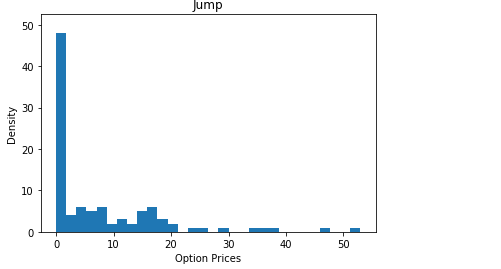
\includegraphics{images/Jump.PNG}
\caption{This is the call payoff from the Jump world, used 252 time
steps, and 100 simulations.}
\end{figure}

\begin{figure}
\centering
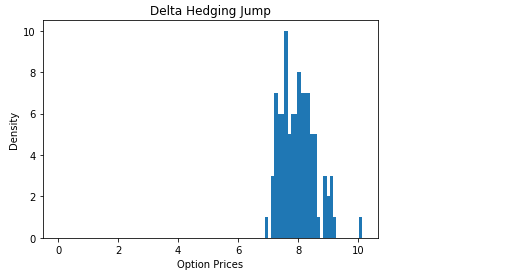
\includegraphics{images/DeltaHedgingJump.PNG}
\caption{This is the call payoff from Jump world with Delta-hedging,
used 252 time steps, and 100 simulations.}
\end{figure}

\begin{figure}
\centering
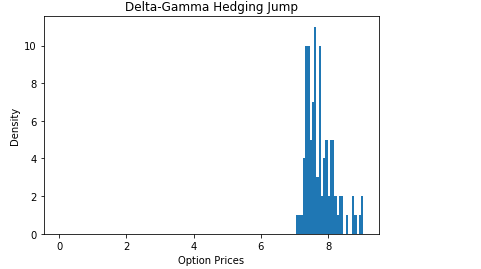
\includegraphics{images/DeltaGammaHedgingJump.PNG}
\caption{This is the call payoff from Jump world with
Delta-Gamma-hedging, used 252 time steps, and 100 simulations.}
\end{figure}

\section{Conclusion}\label{conclusion}

Clewlow and Carverhill bring out the idea that using control variates to
reduce the standard error, also improved the efficiency of Monte Carlo
simulation, combined both perspectives from Finance and Computer
Science. My project is only replicated the process for European call
option, but control variates also good for more complicated path
dependent options, like Asian option, look-back option. In the future, I
am going to combine stochastic volatility to test the real market data.

\newpage
\singlespacing 
\bibliography{./master.bib}

\end{document}
